% This is "sig-alternate.tex" V2.1 April 2013
% This file should be compiled with V2.5 of "sig-alternate.cls" May 2012
%
% This example file demonstrates the use of the 'sig-alternate.cls'
% V2.5 LaTeX2e document class file. It is for those submitting
% articles to ACM Conference Proceedings WHO DO NOT WISH TO
% STRICTLY ADHERE TO THE SIGS (PUBS-BOARD-ENDORSED) STYLE.
% The 'sig-alternate.cls' file will produce a similar-looking,
% albeit, 'tighter' paper resulting in, invariably, fewer pages.
%
% ----------------------------------------------------------------------------------------------------------------
% This .tex file (and associated .cls V2.5) produces:
%       1) The Permission Statement
%       2) The Conference (location) Info information
%       3) The Copyright Line with ACM data
%       4) NO page numbers
%
% as against the acm_proc_article-sp.cls file which
% DOES NOT produce 1) thru' 3) above.
%
% Using 'sig-alternate.cls' you have control, however, from within
% the source .tex file, over both the CopyrightYear
% (defaulted to 200X) and the ACM Copyright Data
% (defaulted to X-XXXXX-XX-X/XX/XX).
% e.g.
% \CopyrightYear{2007} will cause 2007 to appear in the copyright line.
% \crdata{0-12345-67-8/90/12} will cause 0-12345-67-8/90/12 to appear in the copyright line.
%
% ---------------------------------------------------------------------------------------------------------------
% This .tex source is an example which *does* use
% the .bib file (from which the .bbl file % is produced).
% REMEMBER HOWEVER: After having produced the .bbl file,
% and prior to final submission, you *NEED* to 'insert'
% your .bbl file into your source .tex file so as to provide
% ONE 'self-contained' source file.
%
% ================= IF YOU HAVE QUESTIONS =======================
% Questions regarding the SIGS styles, SIGS policies and
% procedures, Conferences etc. should be sent to
% Adrienne Griscti (griscti@acm.org)
%
% Technical questions _only_ to
% Gerald Murray (murray@hq.acm.org)
% ===============================================================
%
% For tracking purposes - this is V2.0 - May 2012

\documentclass{sig-alternate-05-2015}

\usepackage{amsmath}

\begin{document}

% Copyright
% \setcopyright{acmcopyright}
%\setcopyright{acmlicensed}
%\setcopyright{rightsretained}
%\setcopyright{usgov}
%\setcopyright{usgovmixed}
%\setcopyright{cagov}
%\setcopyright{cagovmixed}


% DOI
% \doi{10.475/123_4}

% ISBN
% \isbn{123-4567-24-567/08/06}

%Conference
% \conferenceinfo{PLDI '13}{June 16--19, 2013, Seattle, WA, USA}

% \acmPrice{\$15.00}

%
% --- Author Metadata here ---
% \conferenceinfo{WOODSTOCK}{'97 El Paso, Texas USA}
%\CopyrightYear{2007} % Allows default copyright year (20XX) to be over-ridden - IF NEED BE.
%\crdata{0-12345-67-8/90/01}  % Allows default copyright data (0-89791-88-6/97/05) to be over-ridden - IF NEED BE.
% --- End of Author Metadata ---

\title{{\ttlit Test Case Generation} and {\ttlit Symbolic Execution} using 
Z3\titlenote{Z3 is a high-performance theorem prover. More information about Z3 is
available at \texttt{https://github.com/Z3Prover/z3/wiki}}}
\subtitle{Project Report
\titlenote{This report is part of the project work for \textit{Automated Software Engineering}
course instructed by Dr. Taylor Johnson in Fall, 2015.}}
%
% You need the command \numberofauthors to handle the 'placement
% and alignment' of the authors beneath the title.
%
% For aesthetic reasons, we recommend 'three authors at a time'
% i.e. three 'name/affiliation blocks' be placed beneath the title.
%
% NOTE: You are NOT restricted in how many 'rows' of
% "name/affiliations" may appear. We just ask that you restrict
% the number of 'columns' to three.
%
% Because of the available 'opening page real-estate'
% we ask you to refrain from putting more than six authors
% (two rows with three columns) beneath the article title.
% More than six makes the first-page appear very cluttered indeed.
%
% Use the \alignauthor commands to handle the names
% and affiliations for an 'aesthetic maximum' of six authors.
% Add names, affiliations, addresses for
% the seventh etc. author(s) as the argument for the
% \additionalauthors command.
% These 'additional authors' will be output/set for you
% without further effort on your part as the last section in
% the body of your article BEFORE References or any Appendices.

\numberofauthors{1} %  in this sample file, there are a *total*
% of EIGHT authors. SIX appear on the 'first-page' (for formatting
% reasons) and the remaining two appear in the \additionalauthors section.
%

\author{
% You can go ahead and credit any number of authors here,
% e.g. one 'row of three' or two rows (consisting of one row of three
% and a second row of one, two or three).
%
% The command \alignauthor (no curly braces needed) should
% precede each author name, affiliation/snail-mail address and
% e-mail address. Additionally, tag each line of
% affiliation/address with \affaddr, and tag the
% e-mail address with \email.
%
% 1st. author
\alignauthor
Shafiul Azam Chowdhury\\
       \affaddr{Department of Computer Sc. and Engineering}\\
       \affaddr{The University of Texas at Arlington}\\
       \email{shafiulazam.chowdhury@mavs.uta.edu}
}


\maketitle
\begin{abstract}
This project aims as demonstrating usage of automated software engineering tools. \textit{Z3} is an efficient theorem prover which can be used for automatic test case generation for transition systems and performing symbolic execution of computer programs. I have addressed these two aspects of software engineering in this project. The first task finds test cases for a small sized, multi-state transition system. The second task encodes two interesting computer programs in \textit{Static Single Assignment (SSA)} \cite{Alpern:SSA} form and utilizes Z3 for performing symbolic execution \cite{King:SE}. I perform static analysis on a small computer program and and demonstrate bug-finding approach for an iterative version of the \textit{quicksort} algorithm. 
\end{abstract}


\keywords{Automated software engineering; static analysis; test case generation}

\section{Introduction}
In this project I address two different sort of automated software engineering tasks. In the first task I generate \textit{test cases} automatically for a transition system. This task demonstrates an interesting usage of state of-the art SMT solver; one can use the tool for finding interesting test cases automatically for a transition system. I modeled the popular ``n-puzzle'' game specifying initial states and transition relation of the system. This multiple-state game is ideal for modelling transition relations and safety or liveness requirements. The game begins with one initial state and after some transitions reach a specific goal state. One sort of test cases for the system is finidng those \textit{initial} states from which we can reach the goal state after \textit{x} number of transitions.

I present symbolic execution of interesting computer programs in the second task, which is further organized in two sub tasks. In the first sub-task I analyze a program using symbolic execution to find what inputs cause certain paths of the program to be executed. The second task demonstrates automatic bug finding by encoding a computer program \textit{(quicksort for my project)} into \textit{Static Single Assignment (SSA)} form and negating assertion statements. Z3 the SMT solver can then be utilized to determine if the encoding is satisfiable indicating the system is buggy indeed. By harnessing such static analysis techniques we can perform various automated software engineering tasks in similar projects.

In both of these tasks, I have used Z3 for Python (also known as Z3Py). Z3 is an efficient SMT solver \cite{DeMoura:Z3} developed at Microsoft Research. Z3Py enables us to utilize the powerful features of Z3 in the very popular programming platform - Python. Z3Py can be downloaded from the website \texttt{https://github.com/Z3Prover/z3}.

\section{Test Case Generation for transition system models}

This section describes first task of the project in details. I begin
with presenting a definition of \textit{transition systems} and our
specific problem \textit{n-puzzle} as a transition system. We also
define the task definition that is what do we mean by \textit{test 
case generation}. Next, we focus on creating a formal model of the 
system. A good approach is to first formalize some requirements
of the system which helps identifying the state variables required
to model the system. I then formalize all transition formulae for 
the system. We are then in a position to start implementing the
test case generation problem using Z3Py.

My contribution for this task is an application written in Python 
(which uses Z3 API). The application is complete and parameterized.
The application creates graphical output for the \textit{n-puzzle}
problem, a useful visual aid which demonstrates all of the states
of a game round\footnote{Graphical output is only available when the 
problem is satisfiable i.e. test cases really exist for given parameters.}.  

\subsection{{\subsecit N-puzzle} and transition systems}

We start with an introduction of the n-puzzle game. A more specific 
example would be \textit{15 puzzle} game, which 
consists of a frame of numbered square tiles in random order 
with one tile missing \cite{wiki:npuzzle}. In the 15-puzzle game, these
numbers can any of the numbers from 1 to 15. We say that the board 
has 16 \textit{cells}. No two cell can have the same number. The final
(or goal) state of the game is where the first cell has the number 1,
the second cell has the number 2, and so on. The empty cell should
be at the sixteenth cell. Final state of a 15-puzzle game is shown
in Figure \ref{fig:npfinal}. 

\begin{figure}
\centering
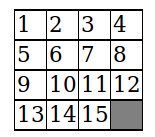
\includegraphics{npfinal}
\caption{Final state of a 15-puzzle game.}
\label{fig:npfinal}
\end{figure}

A game round starts with a \textit{initial} state where cells may have
any values other than the values cell have in the final state. 
After a certain number of \textit{rounds}, the game may go into 
the final state. At any of these rounds, only the empty cell 
is allowed to swap its position with one of its adjacent cells. 
That is, the at each round the empty cell can move only in any the  
upwards, downwards, left of right directions. No other movement of 
cell is allowed. Once the game has reached in the final state, no 
further transitions (movement of the empty cell) are allowed.

Now we are in a position to define the task specifically. Given 
a fixed size of the n-puzzle board, we want to automatically find 
the initial cases from which one may reach the final state making only
\textit{x} transitions. Thus my task falls into the category of test case 
generation problem, where one has to convert the system model into SAT/SMT 
problem and utilize an SMT solver for determining satisfiability.

I chose \textit{n-puzzle} as it is very suitable for modeling in the scope of 
a short-term project. Later I show that this problem falls into the category 
of transition systems, for which we have formal definitions of modeling. A 
transition system has a finite set of typed state variables, a set of initial 
states and a transition description of transitions between states \cite{Alur:CPS}. 

\subsection{Writing System Specifications}
When modeling a transition system, one can start with identifying the state 
variables required for the system and then formalize some of the system's 
requirements. The problem with this approach is, one may end up with unnecessary 
and/or unimportant variables. The alternative is to try formalizing the specifications
first and identify state variables on demand. This approach helps eliminating 
unnecessary vaiables by not creating them at the first time. 

For this reason, we start up with some of the system specifications for \textit{8-puzzle}:

\begin{itemize}
  \item At any state, any cell should have a value greater than 0 and less than or equal to 9.
  We represent the empty cell by the value 9 (16 in a 15-puzzle variant).
  \item No two cell may have the same value.
  \item Only in the final state the cells should have their values ordered, and the system 
  stays in its final round as soon as it reaches there.
\end{itemize}

Once we have identified these specifications, we can determine possible state variables. 
We immediately identifiy that we need one integer variable per cell to keep track which 
number it is representing. Also, we might need a \textit{mode} variable to represent goal 
and non-goal states.

\subsection{Modeling the transition system}

In this section we describe our modeling approach for the transition system. We begin with 
defining some of the transition formulae, and then proceed by specifying implementatio details.

\subsubsection{Transition relations}

Once we have identified possible state variables, we can start defining transition relations. 
For example, for each of the non-goal states, equation \ref{eq:1} represents the transition 
relation showing important constraints, along with other constrains (not shown) to enfore 
system requirements. In the equation, $ cell_i $ represents the value (number) represented by
that cell at step $ i $; $ cell_{i+1} $ represents that cell's value in the next step. $ E $ 
is a symbol for representing the empty cell, which is represented by the number $ 9 $ in a 
$ 3 X 3 $ board. In equation \ref{eq:1}, we represent the right adjacent cell of current cell 
by $ e_{i} $ (``e'' can be considered as shorthand for ``east''). We represent the bottom, left and up 
adjacent cells of the current cell by the symbols $ s_i $, $ w_i $ and $ n_i $ resectively. 
 
\begin{multline} \label{eq:1}
(cell_i = E \wedge \\
  (cell_{i+1} = e_{i} \wedge e_{i+1} = E) \vee \\
  (cell_{i+1} = w_{i} \wedge w_{i+1} = E) \vee \\
  (cell_{i+1} = n_{i} \wedge n_{i+1} = E) \vee \\
  (cell_{i+1} = s_{i} \wedge s_{i+1} = E) \\
))  \vee \\
(
  cell_i != E \wedge ( \\
    (e_{i} = E \wedge e_{i+1} = cell_{i} \wedge cell_{i+1} = E) \vee \\
    (w_{i} = E \wedge w_{i+1} = cell_{i} \wedge cell_{i+1} = E) \vee \\
    (n_{i} = E \wedge n_{i+1} = cell_{i} \wedge cell_{i+1} = E) \vee \\
    (s_{i} = E \wedge s_{i+1} = cell_{i} \wedge cell_{i+1} = E) \vee \\
    (cell_{i+1} = cell_{i})
  )
)
\end{multline}

It should be noted that we have not mentioned all of the required constraints in equation \ref{eq:1}. 
For example, this equation is not applicable directly if current cell is one of the first three cells 
in a $3 X 3$ board, since $n_{i+1}$ represents the top adjacent cell of current cell which is not 
applicable here. We also have not shown other system requirements. For example, in a $3 X 3$ board each 
cell should have one of these values arbitrarily from 1 to 9, and no two cells should have the same 
value. Also note that the value 9 represents the empty cell. 

\subsubsection{Implementation details}

We have used Z3's Python API for modeling the transition system. As mentioned previously, we need one 
integer variable for each of the cells. However, using \textit{Bit-Vectors\footnote{Machine arithmetic 
is available in Z3Py as Bit-Vectors}} instead of integers is recommended as it reduces runtime. Also, 
we need to track value of each cell in each of the steps of the system. We model this requirement using 
\textit{Functions} feature of the Z3Py API. For each cell, we now have one function which takes one 
integer (Bit-Vector) as input and returns one integer (Bit-Vector) as output. the input integer denotes 
the current step, and the output integer denotes value of that cell at that step.

Finally, instead of using a python list to hold the nine functions for each of the nine cells, we use
a two dimensional python list as it enables us to access the cells easily by mentioning two 
indices - representing the ``row'' index and ``column'' index of the cell. The entire model 
is written inside a python class which takes three arugments in its constructor. The first 
argument represents the board size, the second argument denotes number of steps \textit{ (i.e. 
in how many steps we need to reach the goal state)} and the final one puts a bound on how 
many test cases are needed to be generated.


\subsection{Model analyis}

In this section we analyse our implementation of the n-puzzle transition system. We generate 
graphical result showing not only the initial step, but each of the subsequent 
steps of a game round. We generate as many test cases as requested (given such number of test 
cases are available). One such graphical output is presented in Figure \ref{fig:npdemo} where 
the board size is $4 X 4$, two test cases are requested, and the goal state is reached 
in exactly 5 steps.

\begin{figure}
\centering
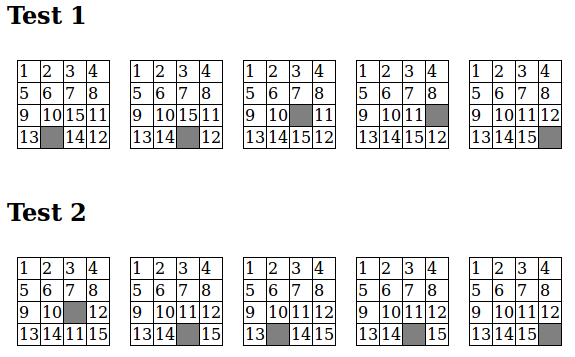
\includegraphics[width=3in]{npdemo}
\caption{Sample result of our implementation of the n-puzzle system. Two test cases
are displayed for a 4X4 board, where the goal state is reached in exactly 5 steps.}
\label{fig:npdemo}
\end{figure}



\subsection{Tables}
Because tables cannot be split across pages, the best
placement for them is typically the top of the page
nearest their initial cite.  To
ensure this proper ``floating'' placement of tables, use the
environment \textbf{table} to enclose the table's contents and
the table caption.  The contents of the table itself must go
in the \textbf{tabular} environment, to
be aligned properly in rows and columns, with the desired
horizontal and vertical rules.  Again, detailed instructions
on \textbf{tabular} material
is found in the \textit{\LaTeX\ User's Guide}.

Immediately following this sentence is the point at which
Table 1 is included in the input file; compare the
placement of the table here with the table in the printed
dvi output of this document.

\begin{table}
\centering
\caption{Frequency of Special Characters}
\begin{tabular}{|c|c|l|} \hline
Non-English or Math&Frequency&Comments\\ \hline
\O & 1 in 1,000& For Swedish names\\ \hline
$\pi$ & 1 in 5& Common in math\\ \hline
\$ & 4 in 5 & Used in business\\ \hline
$\Psi^2_1$ & 1 in 40,000& Unexplained usage\\
\hline\end{tabular}
\end{table}

To set a wider table, which takes up the whole width of
the page's live area, use the environment
\textbf{table*} to enclose the table's contents and
the table caption.  As with a single-column table, this wide
table will ``float" to a location deemed more desirable.
Immediately following this sentence is the point at which
Table 2 is included in the input file; again, it is
instructive to compare the placement of the
table here with the table in the printed dvi
output of this document.


\begin{table*}
\centering
\caption{Some Typical Commands}
\begin{tabular}{|c|c|l|} \hline
Command&A Number&Comments\\ \hline
\texttt{{\char'134}alignauthor} & 100& Author alignment\\ \hline
\texttt{{\char'134}numberofauthors}& 200& Author enumeration\\ \hline
\texttt{{\char'134}table}& 300 & For tables\\ \hline
\texttt{{\char'134}table*}& 400& For wider tables\\ \hline\end{tabular}
\end{table*}
% end the environment with {table*}, NOTE not {table}!

\subsection{Figures}
Like tables, figures cannot be split across pages; the
best placement for them
is typically the top or the bottom of the page nearest
their initial cite.  To ensure this proper ``floating'' placement
of figures, use the environment
\textbf{figure} to enclose the figure and its caption.

This sample document contains examples of \textbf{.eps} files to be
displayable with \LaTeX.  If you work with pdf\LaTeX, use files in the
\textbf{.pdf} format.  Note that most modern \TeX\ system will convert
\textbf{.eps} to \textbf{.pdf} for you on the fly.  More details on
each of these is found in the \textit{Author's Guide}.

\begin{figure}
\centering
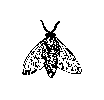
\includegraphics{fly}
\caption{A sample black and white graphic.}
\end{figure}

\begin{figure}
\centering
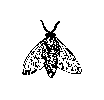
\includegraphics[height=1in, width=1in]{fly}
\caption{A sample black and white graphic
that has been resized with the \texttt{includegraphics} command.}
\end{figure}


As was the case with tables, you may want a figure
that spans two columns.  To do this, and still to
ensure proper ``floating'' placement of tables, use the environment
\textbf{figure*} to enclose the figure and its caption.
and don't forget to end the environment with
{figure*}, not {figure}!

\begin{figure*}
\centering
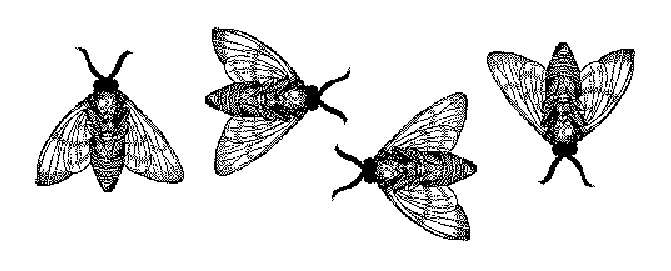
\includegraphics{flies}
\caption{A sample black and white graphic
that needs to span two columns of text.}
\end{figure*}


\begin{figure}
\centering
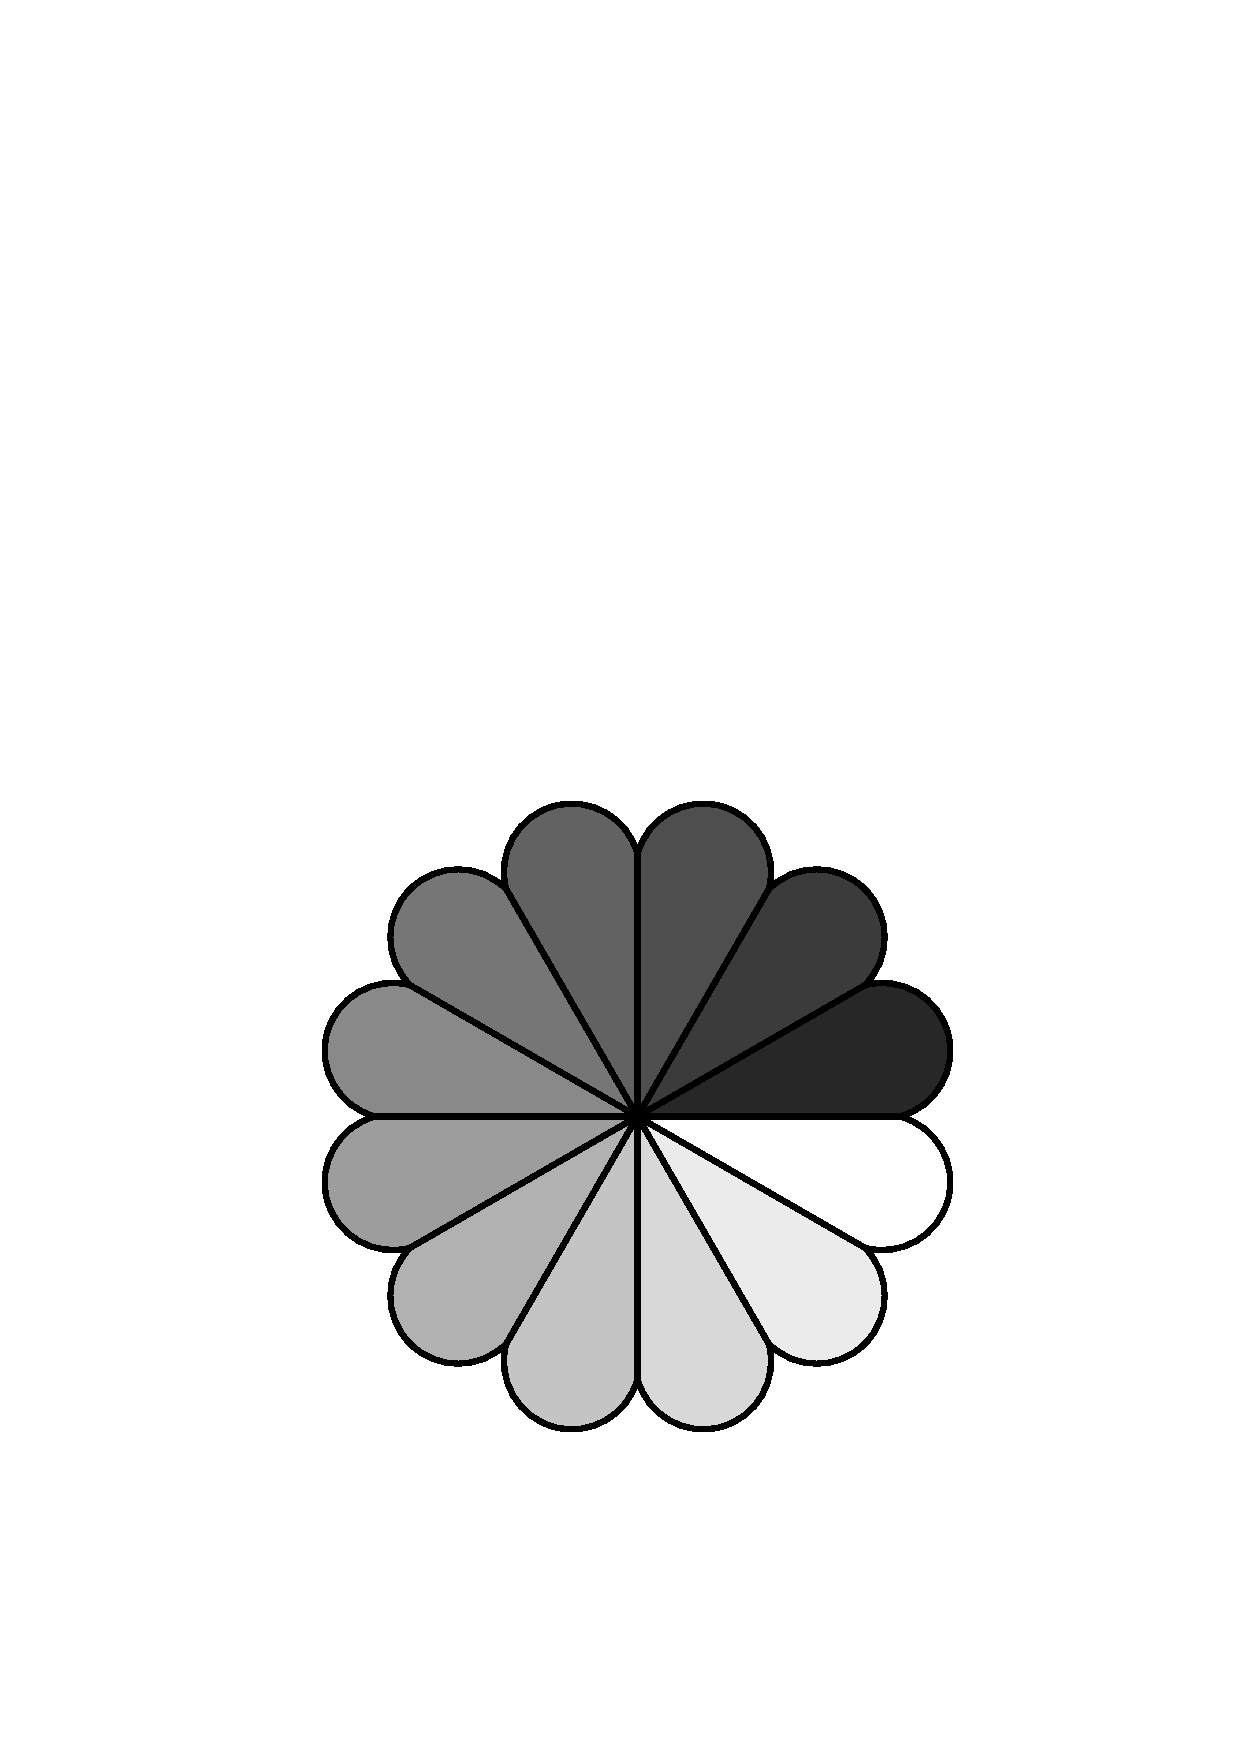
\includegraphics[height=1in, width=1in]{rosette}
\caption{A sample black and white graphic that has
been resized with the \texttt{includegraphics} command.}
\vskip -6pt
\end{figure}

\subsection{Theorem-like Constructs}
Other common constructs that may occur in your article are
the forms for logical constructs like theorems, axioms,
corollaries and proofs.  There are
two forms, one produced by the
command \texttt{{\char'134}newtheorem} and the
other by the command \texttt{{\char'134}newdef}; perhaps
the clearest and easiest way to distinguish them is
to compare the two in the output of this sample document:

This uses the \textbf{theorem} environment, created by
the\linebreak\texttt{{\char'134}newtheorem} command:
\newtheorem{theorem}{Theorem}
\begin{theorem}
Let $f$ be continuous on $[a,b]$.  If $G$ is
an antiderivative for $f$ on $[a,b]$, then
\begin{displaymath}\int^b_af(t)dt = G(b) - G(a).\end{displaymath}
\end{theorem}

The other uses the \textbf{definition} environment, created
by the \texttt{{\char'134}newdef} command:
\newdef{definition}{Definition}
\begin{definition}
If $z$ is irrational, then by $e^z$ we mean the
unique number which has
logarithm $z$: \begin{displaymath}{\log e^z = z}\end{displaymath}
\end{definition}

Two lists of constructs that use one of these
forms is given in the
\textit{Author's  Guidelines}.
 
There is one other similar construct environment, which is
already set up
for you; i.e. you must \textit{not} use
a \texttt{{\char'134}newdef} command to
create it: the \textbf{proof} environment.  Here
is a example of its use:
\begin{proof}
Suppose on the contrary there exists a real number $L$ such that
\begin{displaymath}
\lim_{x\rightarrow\infty} \frac{f(x)}{g(x)} = L.
\end{displaymath}
Then
\begin{displaymath}
l=\lim_{x\rightarrow c} f(x)
= \lim_{x\rightarrow c}
\left[ g{x} \cdot \frac{f(x)}{g(x)} \right ]
= \lim_{x\rightarrow c} g(x) \cdot \lim_{x\rightarrow c}
\frac{f(x)}{g(x)} = 0\cdot L = 0,
\end{displaymath}
which contradicts our assumption that $l\neq 0$.
\end{proof}

Complete rules about using these environments and using the
two different creation commands are in the
\textit{Author's Guide}; please consult it for more
detailed instructions.  If you need to use another construct,
not listed therein, which you want to have the same
formatting as the Theorem
or the Definition\cite{salas:calculus} shown above,
use the \texttt{{\char'134}newtheorem} or the
\texttt{{\char'134}newdef} command,
respectively, to create it.

\subsection*{A {\secit Caveat} for the \TeX\ Expert}
Because you have just been given permission to
use the \texttt{{\char'134}newdef} command to create a
new form, you might think you can
use \TeX's \texttt{{\char'134}def} to create a
new command: \textit{Please refrain from doing this!}
Remember that your \LaTeX\ source code is primarily intended
to create camera-ready copy, but may be converted
to other forms -- e.g. HTML. If you inadvertently omit
some or all of the \texttt{{\char'134}def}s recompilation will
be, to say the least, problematic.

\section{Conclusions}
This paragraph will end the body of this sample document.
Remember that you might still have Acknowledgments or
Appendices; brief samples of these
follow.  There is still the Bibliography to deal with; and
we will make a disclaimer about that here: with the exception
of the reference to the \LaTeX\ book, the citations in
this paper are to articles which have nothing to
do with the present subject and are used as
examples only.
%\end{document}  % This is where a 'short' article might terminate

%ACKNOWLEDGMENTS are optional
\section{Acknowledgments}
This section is optional; it is a location for you
to acknowledge grants, funding, editing assistance and
what have you.  In the present case, for example, the
authors would like to thank Gerald Murray of ACM for
his help in codifying this \textit{Author's Guide}
and the \textbf{.cls} and \textbf{.tex} files that it describes.

%
% The following two commands are all you need in the
% initial runs of your .tex file to
% produce the bibliography for the citations in your paper.
\bibliographystyle{abbrv}
\bibliography{sigproc}  % sigproc.bib is the name of the Bibliography in this case
% You must have a proper ".bib" file
%  and remember to run:
% latex bibtex latex latex
% to resolve all references
%
% ACM needs 'a single self-contained file'!
%
%APPENDICES are optional
%\balancecolumns
\appendix
%Appendix A
\section{Headings in Appendices}
The rules about hierarchical headings discussed above for
the body of the article are different in the appendices.
In the \textbf{appendix} environment, the command
\textbf{section} is used to
indicate the start of each Appendix, with alphabetic order
designation (i.e. the first is A, the second B, etc.) and
a title (if you include one).  So, if you need
hierarchical structure
\textit{within} an Appendix, start with \textbf{subsection} as the
highest level. Here is an outline of the body of this
document in Appendix-appropriate form:
\subsection{Introduction}
\subsection{The Body of the Paper}
\subsubsection{Type Changes and  Special Characters}
\subsubsection{Math Equations}
\paragraph{Inline (In-text) Equations}
\paragraph{Display Equations}
\subsubsection{Citations}
\subsubsection{Tables}
\subsubsection{Figures}
\subsubsection{Theorem-like Constructs}
\subsubsection*{A Caveat for the \TeX\ Expert}
\subsection{Conclusions}
\subsection{Acknowledgments}
\subsection{Additional Authors}
This section is inserted by \LaTeX; you do not insert it.
You just add the names and information in the
\texttt{{\char'134}additionalauthors} command at the start
of the document.
\subsection{References}
Generated by bibtex from your ~.bib file.  Run latex,
then bibtex, then latex twice (to resolve references)
to create the ~.bbl file.  Insert that ~.bbl file into
the .tex source file and comment out
the command \texttt{{\char'134}thebibliography}.
% This next section command marks the start of
% Appendix B, and does not continue the present hierarchy
\section{More Help for the Hardy}
The sig-alternate.cls file itself is chock-full of succinct
and helpful comments.  If you consider yourself a moderately
experienced to expert user of \LaTeX, you may find reading
it useful but please remember not to change it.
%\balancecolumns % GM June 2007
% That's all folks!
\end{document}
